\chapter{Fail-safe Glyph Encoding}
\label{chap:fail_safe}

Glyphs are typically small, and are often designed with a high-degree of similarity in order to facilitate mapping consistency, semantic interpretation, learning, and memorization.
In many applications of spatial or temporal visualization, it is often the case that a large number of small glyphs are required.
From the biological workflows in Chapters \ref{chap:glyph-tax} and \ref{chap:automacron} for instance, the number of glyphs can be in the thousands.
In this chapter we are focused on the \emph{differentiability} of such glyphs and solutions to potential perceptual errors in their observation and exploration.

Figure~\ref{fig:reduction_degradation} presents some example cases that may render some glyphs indistinguishable. 
Zooming out in data exploration can reduce glyph size significantly.
For example, they could make some shapes (\eg, circle and hexagon) and textures appear similar, while confusing the categorization of sizes (\eg, big, medium, small).
Meanwhile, environmental lighting conditions, and printing or photocopying facilities can cause colour and greyscale degeneration.
Such changes would make some glyphs indistinguishable, but may also confuse the association between different colours or shades of grey.
Whilst a dynamic legend may help alleviate the confusion about various mappings, it demands the attention of users through the need to view the legend on a regular basis.
This extra action incurs additional cognitive load due to the effort required for visual search and memorization of the unstable mapping keys.
Other issues could also include colour- or change-blindness, short- or long-sightedness, clustering, occlusion, and distortion.

\begin{figure*}[t]
\begin{center}
%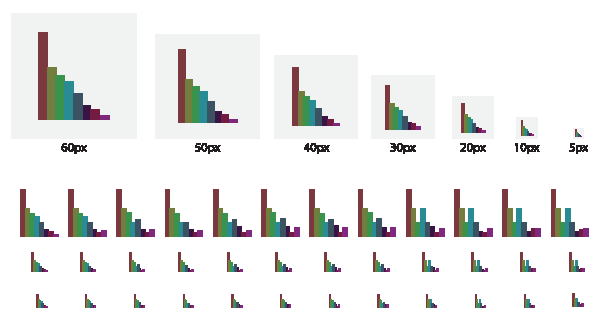
\includegraphics[width=0.9\textwidth, height = 3in]{problems}
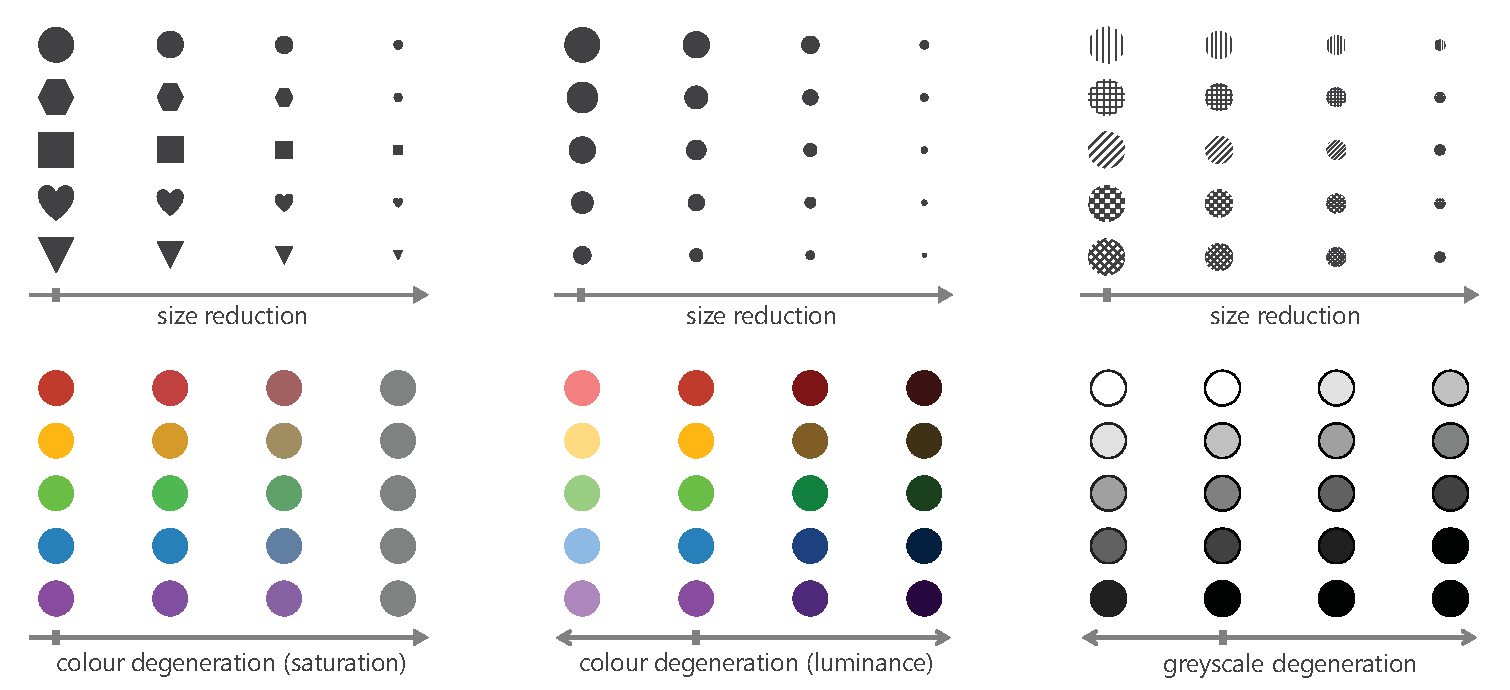
\includegraphics[width=0.95\textwidth]{images/filesystem/Unsafe}
\end{center}
\caption{Three different types of quality degeneration applied to several glyphs, each of which is encoded using a single retinal variable.
The original quality is indicated by a marker on the $x$-axis.
All variations of degeneration result in perception difficulties, however the effect is more so with size, saturation and luminance adjustments.}
\label{fig:reduction_degradation}
\end{figure*} 

Perceptual guidelines discussed throughout this thesis can be adopted for more effective visualization. 
Through using correct data type to retinal variable mappings, prioritizing dimensions based on their importance to tasks, and ensuring separability of dimensions, glyph design can be improved.


%This chapter extends on those foundations to provide a computation
Glyph designers will often apply their creative intuition to ensure the diversity and legibility of different glyphs as is seen within the icon and font design communities.
Much of the work presented in previous chapters has focused on the use of computation in combination with design guidelines to systematize the glyph design process in terms of what retinal variables should be used and where. 
A further research question however would be \emph{``Is there a systematic approach to design a fail-safe glyph set?''}.

In this chapter we propose a conceptual framework to optimize the design of a set of glyphs that provides a systematic way of ensuring fail-safe glyph encoding.
This framework is based on the \emph{Hamming} distance (Section \ref{sec:hamming}).
Due to the perceptual nature of many design aspects, we introduce the conception of the \emph{quasi-Hamming distance} (QHD) (Section \ref{sec:qhd}).
Using this notion, we are able to translate a qualitative assessment of perceptual distances in a design to Hamming distances.
When the minimal Hamming distance for a glyph set is one, the glyph set is vulnerable to ``noise'' during observation and exploration. 
When the minimal Hamming distance is two, the glyph set facilitates some error detection, whereby the viewer can use interaction (\eg, zooming-in, or looking at the legend) to investigate the error.
When the minimal Hamming distance is three or more, the glyph set facilitates some error correction at the receiving end.
This enables us to adjust the design to ensure a minimal Hamming distance among each glyph in a set of glyphs.


To support this novel concept for glyph-based visualization, this work includes the following additional contributions:  
%
\begin{itemize}
\vspace{-2mm}
\item
We outline several methods for estimating QHD, and present two proof-of-concept of experiments for estimating QHD based on the grading by human participants and using image-comparison metrics respectively (Section \ref{sec:qhd}).
\vspace{-2mm}
\item
We present a case study on visualizing file system events, where glyphs were designed to facilitate error detection and correction, and were evaluated by human participants and image-comparison metrics (Section \ref{sec:casestudy}).
\vspace{-2mm}
\item
We demonstrate the uses of the set of fail-safe glyphs to visualize event log data captured from two popular real-world file systems, namely, Dropbox \footnote{\url{www.dropbox.com}} and Git \footnote{\url{www.git-scm.com}} (Section \ref{sec:application}).
The former provides users around the world with file sharing facilities, while the latter is a distributed version control system that supports collaborative software development.
\end{itemize}

\section{Related Work}
\label{sec:relatedworks}

For related work, we consider three topics of interest including: representation of hierarchical and temporal information; glyph-based and event-based visualization; and visualization separability and cognition.

\noindent\textbf{Representation of hierarchical and temporal information}. Originally proposed by Johnson and Shneiderman~\cite{johnson91}, Treemaps have proven a popular technique for visualizing hierarchical data, such as file systems, using a nested rectangle approach.
In the literature, there is much work that aims to extend upon this by increasing the capacity of data that can be visualized, and the addition of temporal information.
Tu and Shen propose using contrast Treemaps to depict change between two or more snapshots of hierarchical data~\cite{tu07}.
Card~\etal introduce \textit{TimeTree}, which allows a user to interactively browse temporal change in hierarchical data~\cite{card06}.
Lamping and Rao propose the use of a hyperbolic browser for visualizing large hierarchical data that incorporates a fish-eye lens to provide focus and context~\cite{lamping96}.
Holten extends this approach to show hierarchical edge bundles that depict relationships between data points~\cite{holten06}.
Burch and Diehl introduce \textit{TimeRadarTress}, that use a radial tree layout to depict hierarchy, with associated circle sectors to also show temporal changes~\cite{burch08}.
Ther\'{o}n also uses a radial layout, based on a tree-ring metaphor for depicting hierarchical data whilst also incorporating the temporal element~\cite{theron06}.
More recently, Guerra-G\'{o}mez~\etal introduced \textit{TreeVersity2} for visualizing temporal changes in dynamic hierarchical data~\cite{guerragomez13}.

\noindent\textbf{Glyph-based and event-based visualization}. Glyph design has been discussed extensively in Chapter \ref{chap:glyph-tax} and is shown to be a popular way of visualizing event-based visualizations due to its ability to represent many variables at once, and preserve spatial information.
For example, Kapler and Wright developed a prototype system \textit{GeoTime} that displays military events in a combined temporal and geo-spatial visualization~\cite{kapler04}.
Gatalsky~\etal use the similar concept of the ``space-time cube'' to visualize spatio-temporal information relating to earthquake events~\cite{gatalsky04}. 
Pearlman and Rheingans use glyphs for visualizing network security events~\cite{pearlman08}. 
Suntinger~\etal~\cite{suntinger08} also use glyph-based event visualization to create an \textit{Event Tunnel} for business analysis and incident exploration.
J\"{a}nicke~\etal~\cite{janicke10} developed \textit{SoundRiver} that mapped movie audio/video content to glyph visualizations on a timeline.
Ware and Plumlee~\cite{Ware01072013} investigated the use of glyph-based visualization for encoding multivariate weather data such as temperate, pressure, wind direction, and wind speed.
Wongsuphasawat~\etal introduce \emph{LifeFlow} as a scalable interactive overview of temporal event sequences~\cite{wongsuphasawat11}.
Ferreira~\etal visualize spatio-temporal events for assessing New York taxi trips~\cite{ferreira13}.
Luo~\etal visualize events in automated text analysis from large text collections, using their proposed system \textit{Event River}~\cite{luo12}.
Additionally, storyboard visualization has become popular for depicting key events in temporal data such as movie content~\cite{tanahashi12, liu13}.


\noindent\textbf{Visualization separability and cognition}. Chen and J\"{a}nicke~\cite{Chen:2010:TVCG} proposed an information-theoretic approach that compares the process of developing visualizations with the traditional communication model.
Chen~\cite{chen08} discusses an information theoretic viewpoint for the development of visual analytics tools.
Duke~\etal~\cite{duke05} discuss the importance surrounding interpretation, examining how viewers could potentially perceive different meanings from the same visualization.
Liu~\etal~\cite{liu08} presented distributed cognition as a theoretical framework for visualization.
van Wijk~\cite{vanwijk05} discusses the value of visualization, and how it is a combination of art, science, and the real world.
As part of our interest in separability, there are numerous image comparison metrics that have been proposed in the image processing literature (\eg, \cite{Sahasrabudhe99, Eler08}).
Such metrics have also been adopted in visualization, where Zhou~\etal~\cite{Zhou:2002:Vis} studied eleven metrics for comparative visualization.
Daniel and Chen~\cite{Daniel:2003:Vis} also studied image comparison metrics for video visualization.
Recently, Schmidt~\etal~\cite{Schmidt:2013:TVCG} developed an interactive web application for supporting image comparison.

\section{Hamming Distance}
\label{sec:hamming}

\begin{figure}[h!]
\begin{center}
\includegraphics[width=\textwidth]{images/filesystem/latest/Hamming1}
\end{center}
\caption{Principles of error correcting codes.
A) A code with no error detection where every code is valid. No way of detecting errors and no way of correcting them.
B) A code with a distance of two bits between valid codes can detect errors but cannot correct since one change in any position will result in a valid code (knowing what changed is difficult).
C) A code with a distance of three bits between valid codes can detect errors and correct them.}
\label{fig:hamming}
\end{figure}


In information theory and data communication, a \emph{code} consists of a finite set of \emph{codewords}, each of which is a digital representation of a letter in an alphabet.
In the context of binary encoding, the \emph{Hamming distance}, proposed by Richard Hamming in 1950 \cite{Hamming:1950:Bell}, is a measure of the number of bit positions in which two codewords differ.
Considering all pairs of codewords in a code, the minimal distance is referred to as the minimal Hamming distance of the code (In the literature, the word minimal is often confusingly omitted).
In communication, there are two main strategies for dealing with errors that occur during transmission.
\emph{Automated error detection} allows the receiver to discover that any error has occurred and to request a retransmission accordingly.
\emph{Automated error correction} enables the receiver to detect an error and deduce what the intended transmission must have been.
Hamming defined the following principle:

\noindent \textbf{Theorem.} A code of $d+1$ minimal Hamming distance can be used to detect $d$ bits of errors during transmission. A code of $2d+1$ minimal Hamming distance can be used to correct $d$ bits of errors during transmission~\cite{Hamming:1950:Bell}.

For example, given a 3-bit code as illustrated in Figure~\ref{fig:hamming}, there are 8 possible codewords.
One may select a subset of these codewords to construct a code with its minimal Hamming distance equal to two bits or three bits.
Figure~\ref{fig:hamming} B) shows such a code with four valid codewords and is of two bits minimal Hamming distance.
This code can detect 1-bit errors since any change of a valid codeword by 1 bit would result in an invalid codeword, which would lead the receiver to discover the error.
Figure~\ref{fig:hamming} C) shows another code, with two valid codewords and is of 3 bits minimal Hamming distance.
This code can detect 2-bit errors and correct one-bit errors.
When a valid codeword (\eg, 111) is changed by 1 bit during transmission (\eg, 110), the receiver can detect such an error and recover the intended codeword based on the nearest neighbour principle.
Of course, if a 2-bit error occurred during transmission, the receiver would be able to detect the error but could not make a correct ``correction''.
Nevertheless, if it is known that two-bit errors are likely to occur then this should either be used as only an error detection code, or a code with a longer Hamming distance should be used instead.

\begin{figure}[t]
\begin{center}
\includegraphics[width=0.85\textwidth]{images/filesystem/latest/QHD}
\end{center}
\caption{Two examples that illustrate the phenomena of error detection and error correction in glyph-based visualization. (Above) A viewer may sense that the glyph on the left may not be correct in a distorted visualization, and consult the legend to correct the error. (Below) A viewer may unconsciously perceive the glyph on the left as a star shape due to Gestalt effects and apriori knowledge about the glyph set.}
\label{fig:glyph_hamming}
\end{figure}

\section{Quasi-Hamming Distance for Glyph Design}
\label{sec:qhd}
%
A set of glyphs is a code, and each glyph in the set is a valid codeword.
On presenting a glyph-based visualization to a user, there may be errors in the display and perception of a glyph.
If a viewer can detect that a perceived glyph is not quite ``right'', conscious or unconscious effort can be made to correct such an error.
Conscious effort, which is an analogy of error detection and repeated transmission, may typically include zooming in to have a close look, or consulting the legend.
Unconscious effort, which is an analogy of error correction, may include some Gestalt effects \cite{Chen:2014:CGF}, and inference from other visual information \cite{Rheingans:1995:PIV}.
Figure~\ref{fig:glyph_hamming} shows two example glyph sets, each with eight codewords.
Given the two display errors shown on the left, \emph{i.e.}, an arrow glyph is skewed in a distorted printout, and a shape glyph is occluded by another shape.
Both errors can be detected, although the error for the arrow glyph will require more conscious effort to correct, although in this case that would be impossible due to the small distance between glyph in the set. 
The star glyph can be corrected unconsciously due to Gestalt effects in combination with the greater distance between each of the glyphs in the set.
These examples would suggest that it is possible to establish a conceptual framework, similar to the Hamming distance for error detection and error correction in glyph-based visualization.

Understandably, measuring the distances and errors in visual perception is not as simple as measuring those represented by binary codewords.
We thereby propose an approximated conceptual framework based on the principle of Hamming distance, which we call a \emph{Quasi-Hamming Distance} (QHD).
The term ``quasi'' is used to show that the distance measure is an approximate, and that the quantitative measure of perceptual error is also approximated.
Therefore the main research questions are:
i) can we establish a measurement unit common to both measures?; and
ii) given a glyph set, how can we measure the distance between those glyphs?\\

\noindent\textbf{Can we establish a measurement unit common to both measures?} We can utilize a ``bit'' as the common unit for both distance and error measurement.
Consider an ordered retinal variable, such as brightness or length, as a code $C$.
Theoretically $C$ can have a set of codewords $\{ c_1, c_2, \ldots c_n \}$ such that the difference between two consecutive codewords is the just-noticeable difference (JND) of this retinal variable.
We can define the QHD between each pair of codewords $c_i$ and $c_j$ as $|i-j|$ bits.
During display and visualization, if $c_i$ is mistaken for $c_j$, we can call this a $d$-bit error where $d=|i-j|$.
Now let us extend this concept to a less ordered retinal variable (\eg, colour hue).
Theoretically, we can construct a code $C$ by uniformly sampling the space of the retinal variable (\eg, the CIE L*a*b* colour space) while ensuring that every pair of samples differ by at least the JND of this channel.
These codewords can be organized into a network, where the distance between any two codewords can be approximated proportionally according to the JND (\emph{i.e.}, JND = 1 bit).
Note that the possible perception error rate with a code that maximizes the number of codewords based on JND is likely to be very high.
In practice, one designs a glyph set based only on a small subset of samples of a retinal variable or more commonly in the multivariate space of several retinal variables.
Hence a QHD measure based on JND would be too fine to use in practice, though longer term, JND can provide an \emph{absolute reference measure} once we have obtained measures for the majority of retinal variables used in visualization.\\

\noindent\textbf{Given a glyph set, how can we measure the distance between glyphs?} One may consider using the following methods:
\begin{enumerate}
\vspace{-1mm}
\item \textbf{Estimation by expert designers.} This practice has existed in design exercises such as the development of traffic signage (discussed in Chapter \ref{chap:related_work}, Section \ref{sec:relwork_glyphs}) and icons in user interfaces.
To formalize this practice, designers can explicitly estimate and label the distance between each pair of glyphs in a glyph set.
While this approach may be most convenient to the designers, its effectiveness depends very much on the experience of the designers concerned and it is easy to overlook certain types of display and perception errors;
\vspace{-1mm}
\item \textbf{Crush tests.} This test was introduced in Chapter \ref{chap:glyph-tax} to simulate how changes in size affect the perception of glyph features.
By simulating the various causes of perception error, such as those illustrated in Figure~\ref{fig:reduction_degradation}, we can determine the level at which glyphs become indistinguishable.
The corresponding level of degeneration can be defined as a QHD.
While this approach would yield more consistent estimation of a QHD, more research would be required to compile a list of different causes of errors and define coherent levels of degeneration across different causal relationships;
\vspace{-1mm}
\item \textbf{Task-based evaluation.} Similar to (2), one can simulate different visualization conditions, enlist users to perform their tasks, measure their performance, and transform performance measures to a QHD.
On one hand, this approach is perhaps most semantically meaningful for a particular glyph set in a specific application context.
On the other hand, the performance measures collected may feature many confounding effects, while there may only be a small number of users available for such an evaluation.
\vspace{-1mm}
\item \textbf{User-centric estimation.} One may conduct a survey among human participants about how easy or difficult to differentiate different glyphs. By removing task-dependency in (3), more participants can be involved in such a survey, yielding a more reliable estimation of the QHD.
Recent efforts have taken place to crowd source distances between simple shapes, colours, and sizes to create what are called \emph{Perceptual Kernels} \cite{demiralplearning}.
\vspace{-2mm}
\item \textbf{Computer-based similarity measures.} There exists a large collection of image similarity measures in the literature~\cite{Sahasrabudhe99, Eler08}.
It is likely that we will be able to find measures that are statistically close to a user-centric estimation in the long term.
However, short term, there are few metrics specially designed for measuring the similarity of glyphs.
\end{enumerate}

To demonstrate the feasibility of estimating a QHD, we conducted two proof-of-concept experiments based on methods (4) and (5).
We conducted a survey among twenty participants, all of whom are either employees or students at University of Oxford.
About 50\% encountered glyph-based visualization in their course or work.
The results of one participant were considered as an outlier and were not included in the statistics.
After a brief introduction, the participants were asked to rate how difficult or easy it was to differentiate 104 pairs of glyphs using an integer scale from 0 to 10.
The survey was conducted during an informal lunch, where pizzas were served.
No cash payment was involved.

\begin{figure*}[h!]
\begin{center}
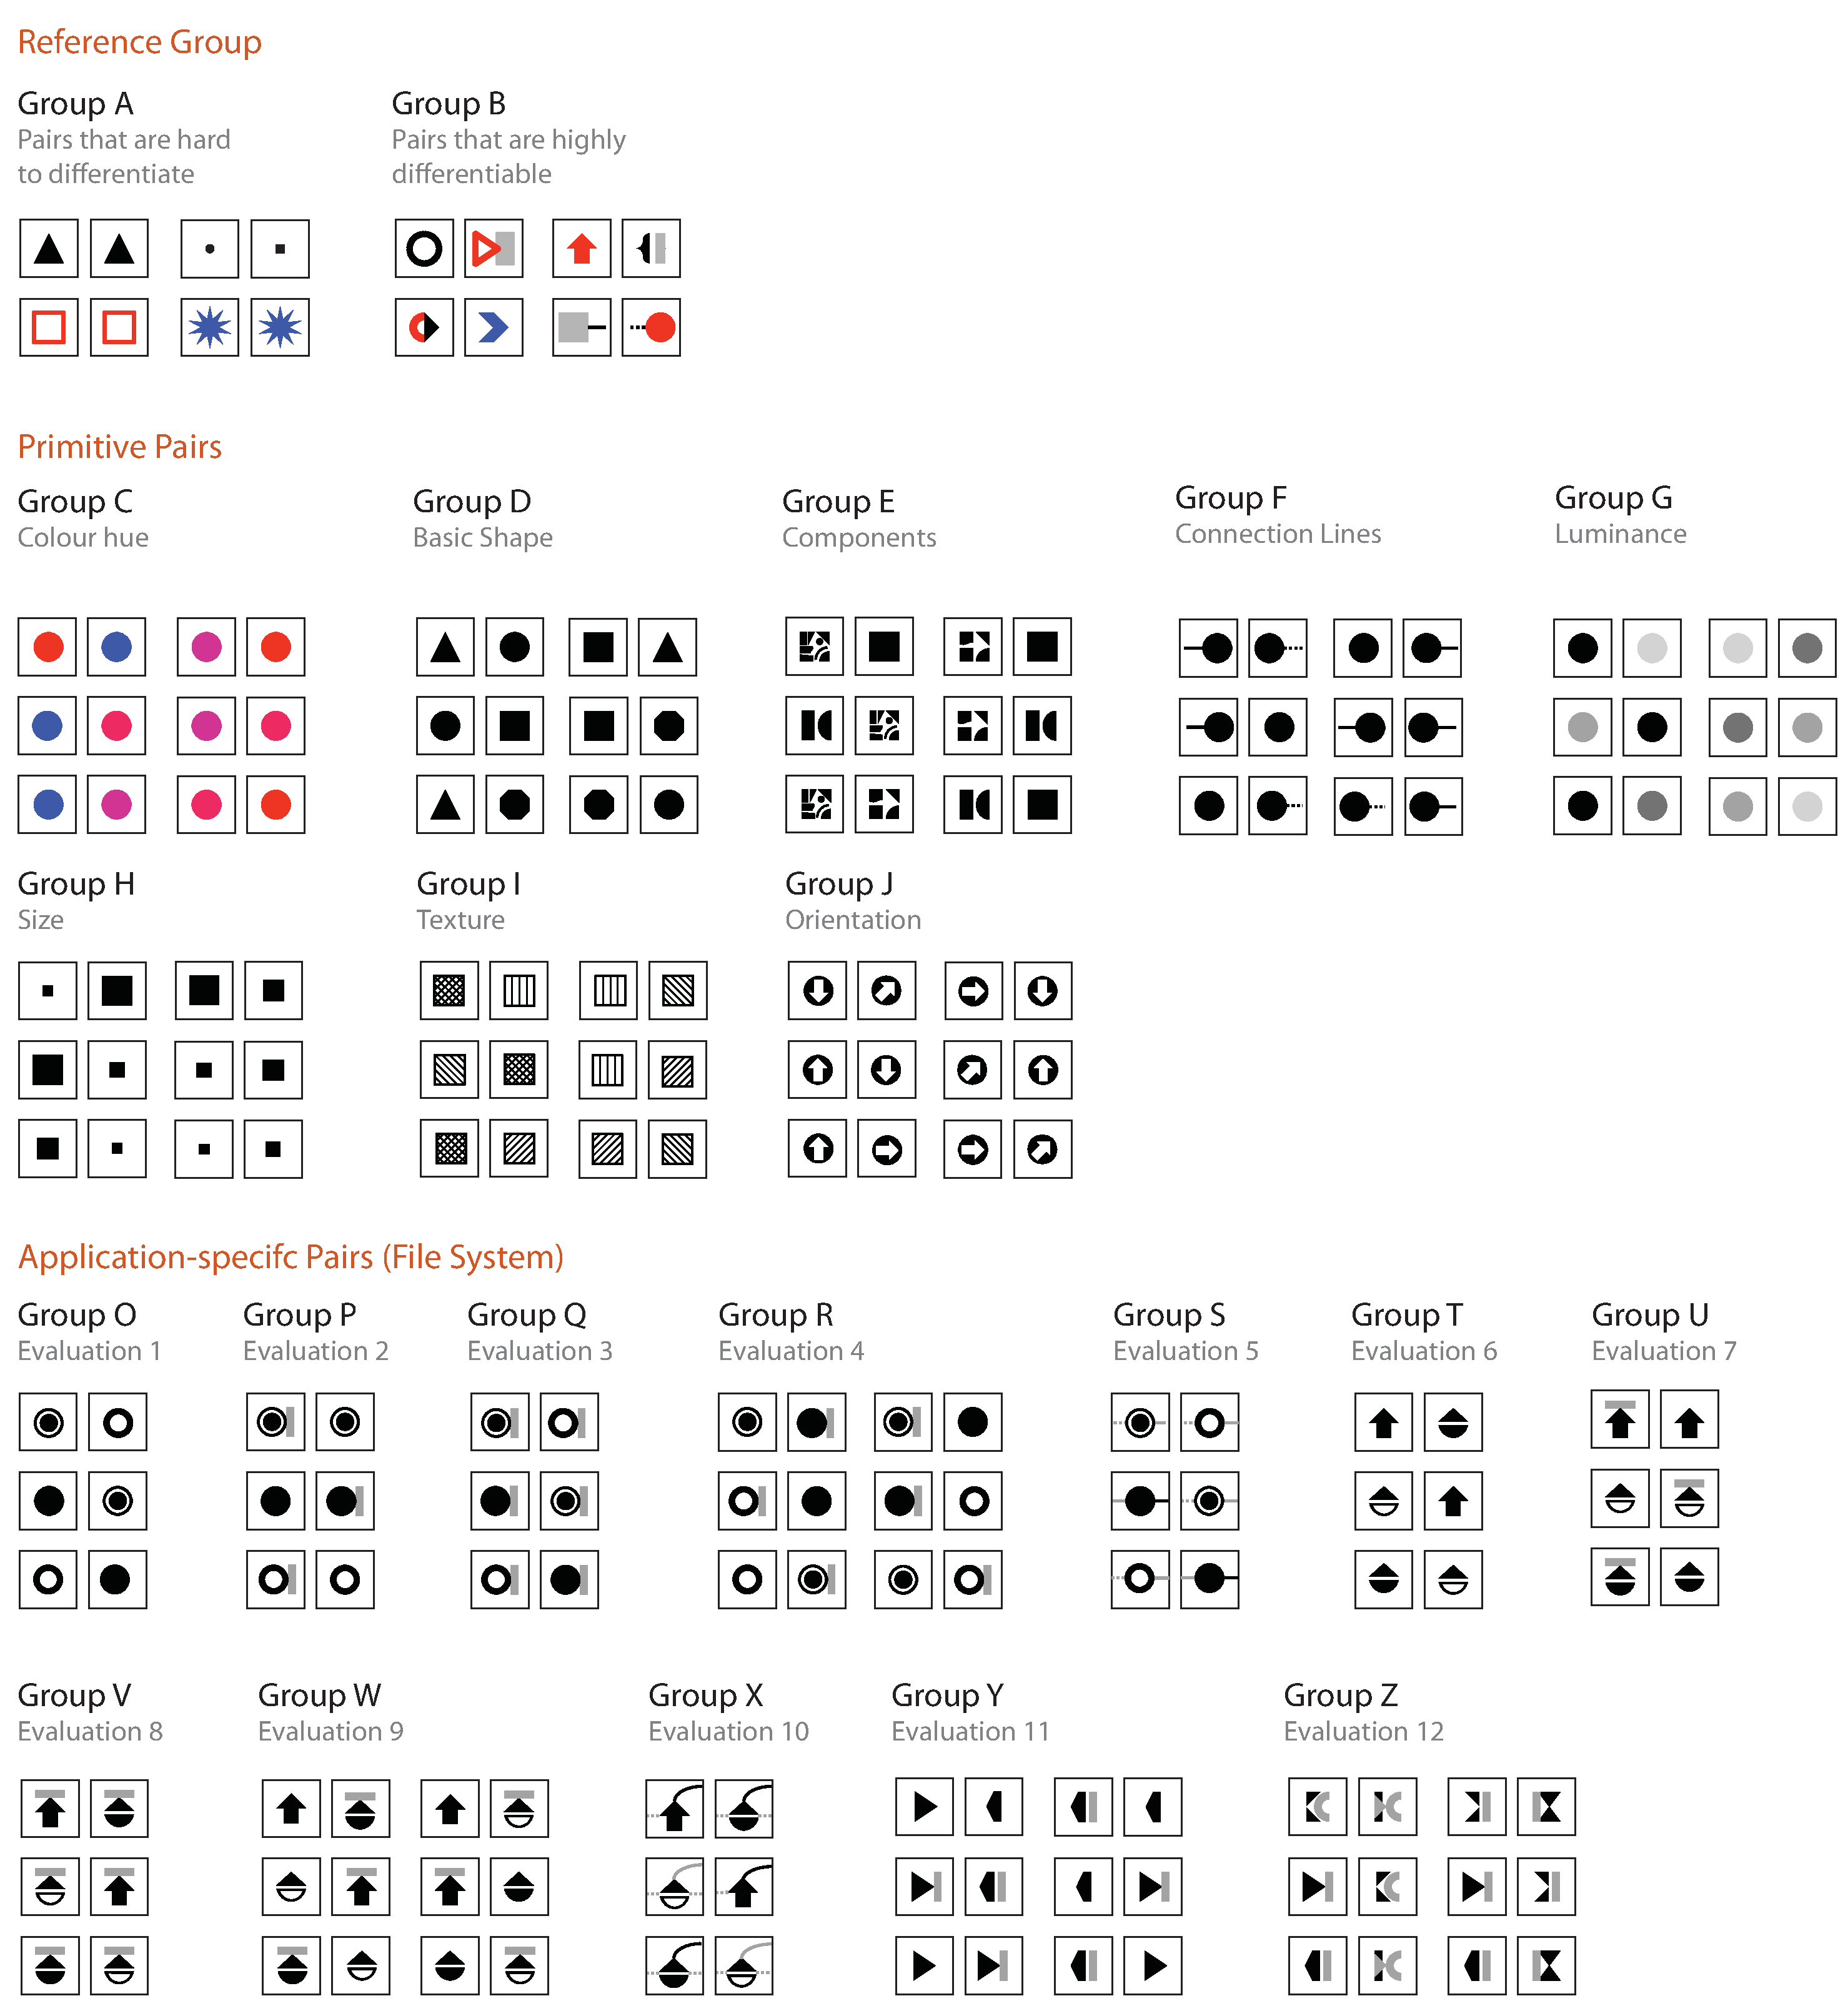
\includegraphics[width=\textwidth]{images/filesystem/evaluation_groups}
\end{center}
\caption{104 stimulation pairs are split in to three groups representing: the reference group; primitive pairs; and application-specific pairs.}
\label{fig:evaluation_groups}
\end{figure*}


Illustrated in Figure \ref{fig:evaluation_groups} are the 104 stimuli pairs divided into three categories: eight \emph{reference pairs}; forty-eight \emph{primitive pairs}; and forty-eight \emph{application-specific pairs}.
We will discuss the last category in detail in Section \ref{sec:application}.
The ninety-six primitive and application-specific pairs were mixed together in a randomized order.
The eight reference pairs were placed at positions 1, 2, 35, 36, 69, 70, 103, and 104 for helping participants to regularize their scores and for enabling us to check temporal consistency.
Here we briefly describe the survey results in relation to the reference and primitive pairs.

The category of reference pairs are divided into two groups.
Group A consists of four pairs of very similar glyphs, and Group B consists of four pairs of very different glyphs. 
We expected that participants would assign very low scores (difficult to differentiate) to those in A and high scores (easy to differentiate) to those in B respectively. As mentioned earlier, we placed one pair from A and one from B at regular intervals.
The average scores for the four pairs in group A are (0.0, 0.4, 1.4 and 2.8) respectively and those for group B are (9.3, 9.0, 8.9, 9.7) respectively, indicating that they have statistically served as references for the minimal and maximum QHD in this survey.

The category of primitive pairs consists of eight groups for estimating QHD in relation to eight retinal variables, namely colour hue, shape, components, connection lines, luminance, size, texture, and orientation.
Each group has six pairs of stimuli, facilitating pairwise comparison of four different codewords of each channel.
For hue and luminance channels, after choosing the first and fourth codewords we used a perceptually uniform colour model (Hunter's Lab) to determine the second and third codewords at 50\% and 75\% distance from the first.
The upper part of Figure~\ref{fig:eval_glyph_scores} shows a small selection of survey results, where we converted the $[0, 10]$ score range to a $[0, 5]$ QHD range, and we considered that any QHD $<2$ is potentially risky for error detection, and any QHD $<3$ is potentially risky for error correction.

\begin{figure*}[h!]
\begin{center}
\includegraphics[width=\textwidth]{images/filesystem/latest/Comparison}
\end{center}
\caption{Sample of results for the primitive glyph pairs used in both the user-centric estimation (top) and by computer-based similarity measure (bottom). Low values indicate difficult to differentiate and high values indicate easy to differentiate.}
\label{fig:eval_glyph_scores}
\end{figure*}

In our second experiment, we measured the similarity between each pair of glyphs using a computer-based metric.
This metric combines differences in pixel colour with spatial occupancy.
The former captures a variety of feature differences such as colour, luminance, size, and orientation, \emph{etc.} and is defined as the mean Euclidean distance between all corresponding pixels in the two images representing the pair of glyphs.
The latter captures some location-invariant features such as spatial occupancy and additional components, and is defined as the difference between the numbers of pixels with $\leq 80\%$ luminance.
Both difference measures are first normalized to the $[0, 1]$ range, and are then scaled to the same QHD range as the survey (with the same min, mean, max), before being combined into a single metric.
The lower part of Figure~\ref{fig:eval_glyph_scores} shows the computed similarity measures for the same selection of stimuli pairs.

\begin{figure*}[t]
\begin{center}
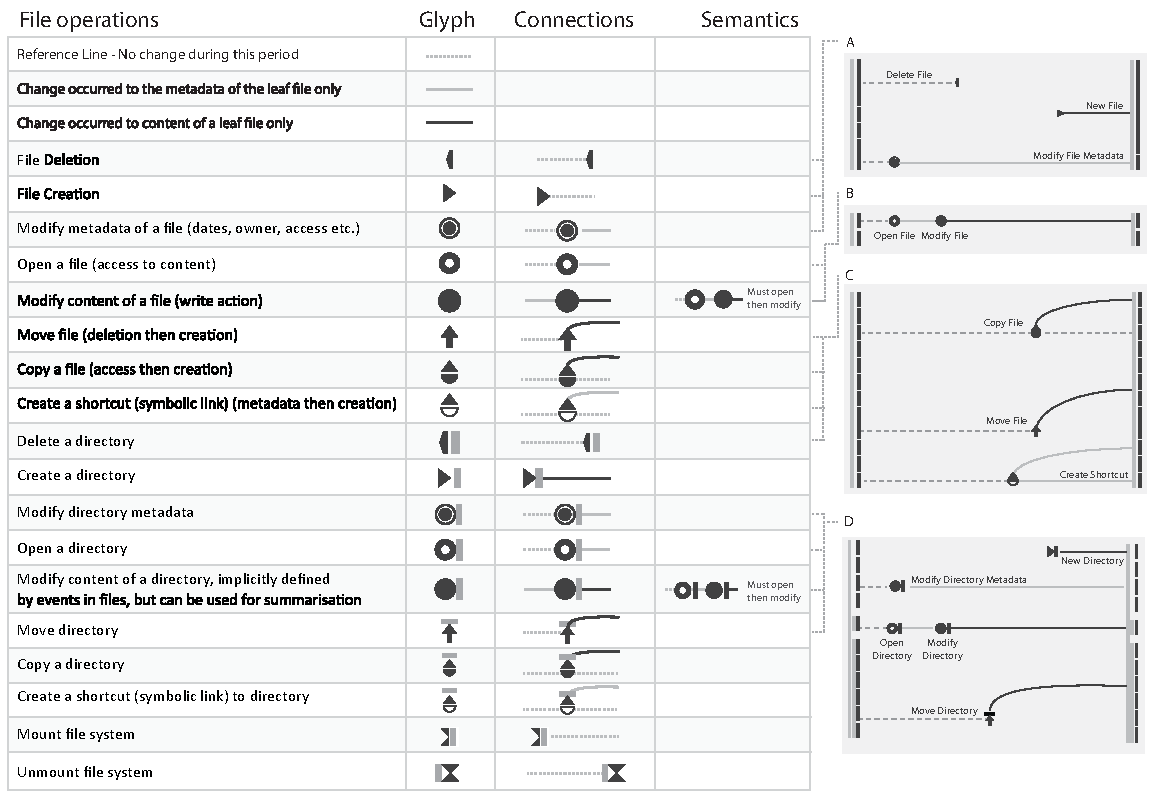
\includegraphics[width=0.99\textwidth]{images/filesystem/table_new}
\end{center}
\caption{Eighteen glyphs designed to represent different events in file systems.
Each event is associated with its primary glyph representation in the second column.
In addition, an event may be associated with special signatures in terms of connection (in the third column) and semantic ordering (in the fourth column).}
\label{table:fileoperations}
\end{figure*}

\section{Case study: Visualizing File System Events}
\label{sec:casestudy}

The problem of visualizing file systems plays a significant role in the short history of computer-assisted visualization.
In 1991, Johnson and Shneiderman, who were motived by the need to visualizing the structure of a file system, published their seminal paper on treemaps~\cite{johnson91}.
Today, not only are file systems much larger and contain many more files, they are also shared by many more users and have many more events.
One important aspect of a file system is to support collaborative activities, such as sharing files within multi-partner projects and developing software by a team of programmers.
While there are text-based mechanisms for recording events in relation to a file system or a specific folder, the amount of data contained in typical log files can easily escalate to the point where it becomes too overwhelming for anyone to read on a regular basis until perhaps some disastrous events take place.
To our knowledge, there is no effective visualization technique for allowing users of such collaborative environments to observe events in a cost-effective manner.

In this case study, we designed and developed a novel glyph-based visualization tool for observing events in a file system.
There are several technical challenges.
Firstly, the hierarchical nature of the file system needs to be depicted so that the spatial context of where a particular event has occurred can be identified.
Secondly, the temporal information about events needs to be conveyed so that the activity ordering can also be observed and reasoned.
Thirdly, there are a wide range of activities (\eg, copying a file, modifying a file) that are typically performed, which would need to be distinguishable in a visualization.
Finally, the visualization should be able to support collaborative environments by depicting activities from different users.

\begin{figure*}[h]
\begin{center}
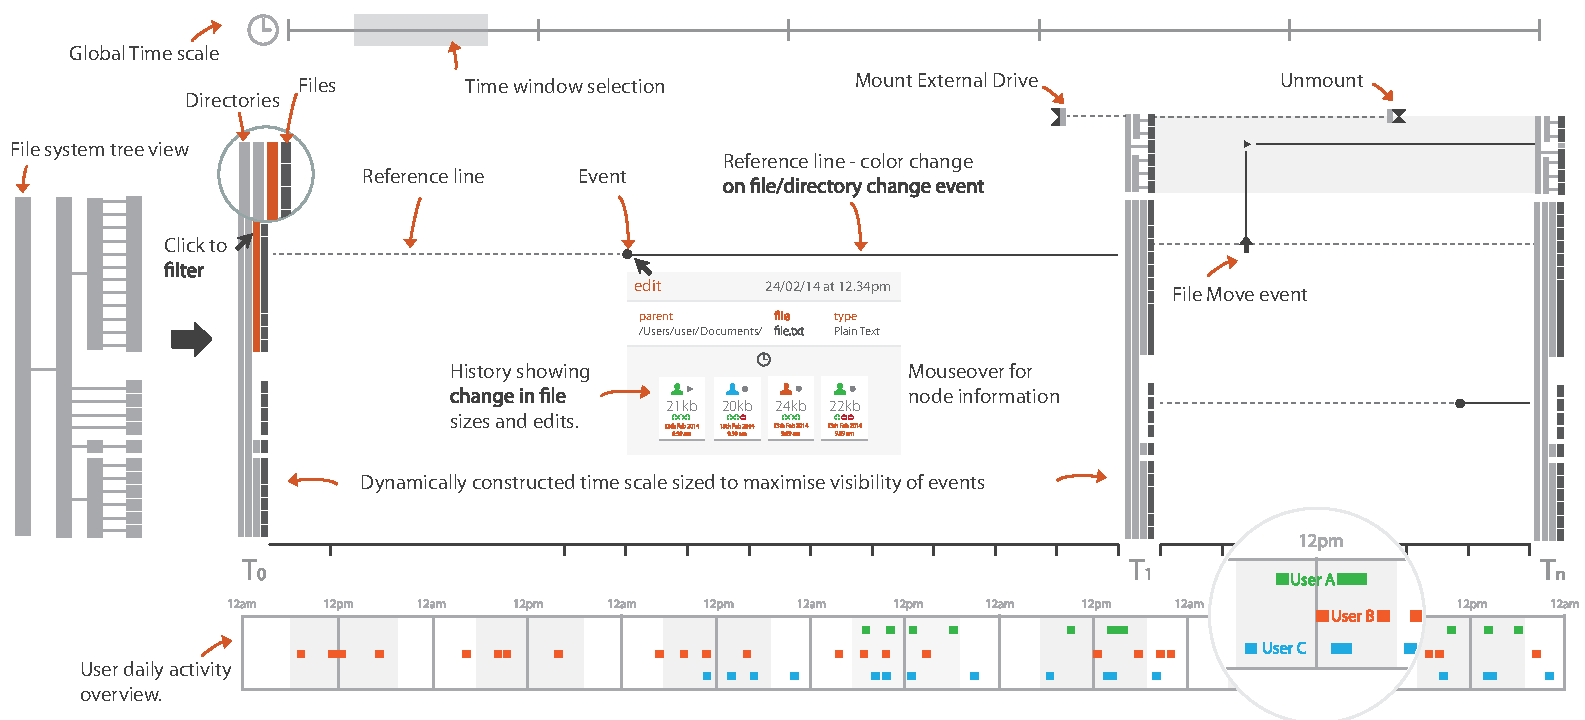
\includegraphics[width=\textwidth]{images/filesystem/system_overview}
\end{center}
\caption{Visualization overview. We use a timeline approach with a condensed file system hierarchy at the left of the visualization. File system activities are depicted by glyphs on the timeline, with connected lines to show correspondence to the file system. Keyframes are displayed to depict significant changes to the file system hierarchy, or at user-specified time intervals. Interation with mouse cursor displays context box with detailed information on the selected file, directory, or activity.}
\label{fig:system}
\end{figure*}

Figure~\ref{fig:system} presents an overview of the visualization and the design process that was adopted for the layout.
The visualization layout consists of a number of different components that we shall discuss.
The central area of the visualization is the main activity window where the events performed on the file system are displayed on a timeline using glyph-based visualization. 
The glyphs that have been designed for this application are discussed in detail in the next section.
To the left of the main activity window is the file system tree view, which represents the file system using a traditional tree representation where directories are shown as light gray nodes and files shown as dark gray nodes.
Since most directories are likely to contain files, leaf nodes are typically file objects.
This tree is shown as a condensed display to the left of the main timeline and serves as a reference to spatial context of the file location.
File system events in the main window are positioned in correspondence to the file system hierarchy.
Connected lines are displayed to relate the file activities back to the particular file in the hierarchy.
For events that involve a change in the file system hierarchy, such as copying or moving files, these connecting lines also indicate the new position of the file.
The condensed file hierarchy also serves as a ``keyframe'', where the current state of the file system hierarchy is shown, either after a significant change to the hierarchy (\eg, copying files, or mounting an external drive), or at a particular time interval specified by the user.
Finally, the file hierarchy can also be used to select the directory of interest that should be shown on the visualization.
This provides a mechanism for ``zooming in'' to a particular directory, or ``zooming out'' to view the root directory.
At the top of the display is a time window selection bar, that allows the user to specify the time period that should be shown in the main activity window. 
At the bottom of the display is a daily activity overview that provides a summary of which users have perform some event and at what time.
The interface also supports a pop-up window that is displayed as the mouse hovers over a particular event. 
The window provides more information that is related to both the current event, and the file.

\subsubsection{Designing Event Glyphs}

\begin{figure*}[t!]
\begin{center}
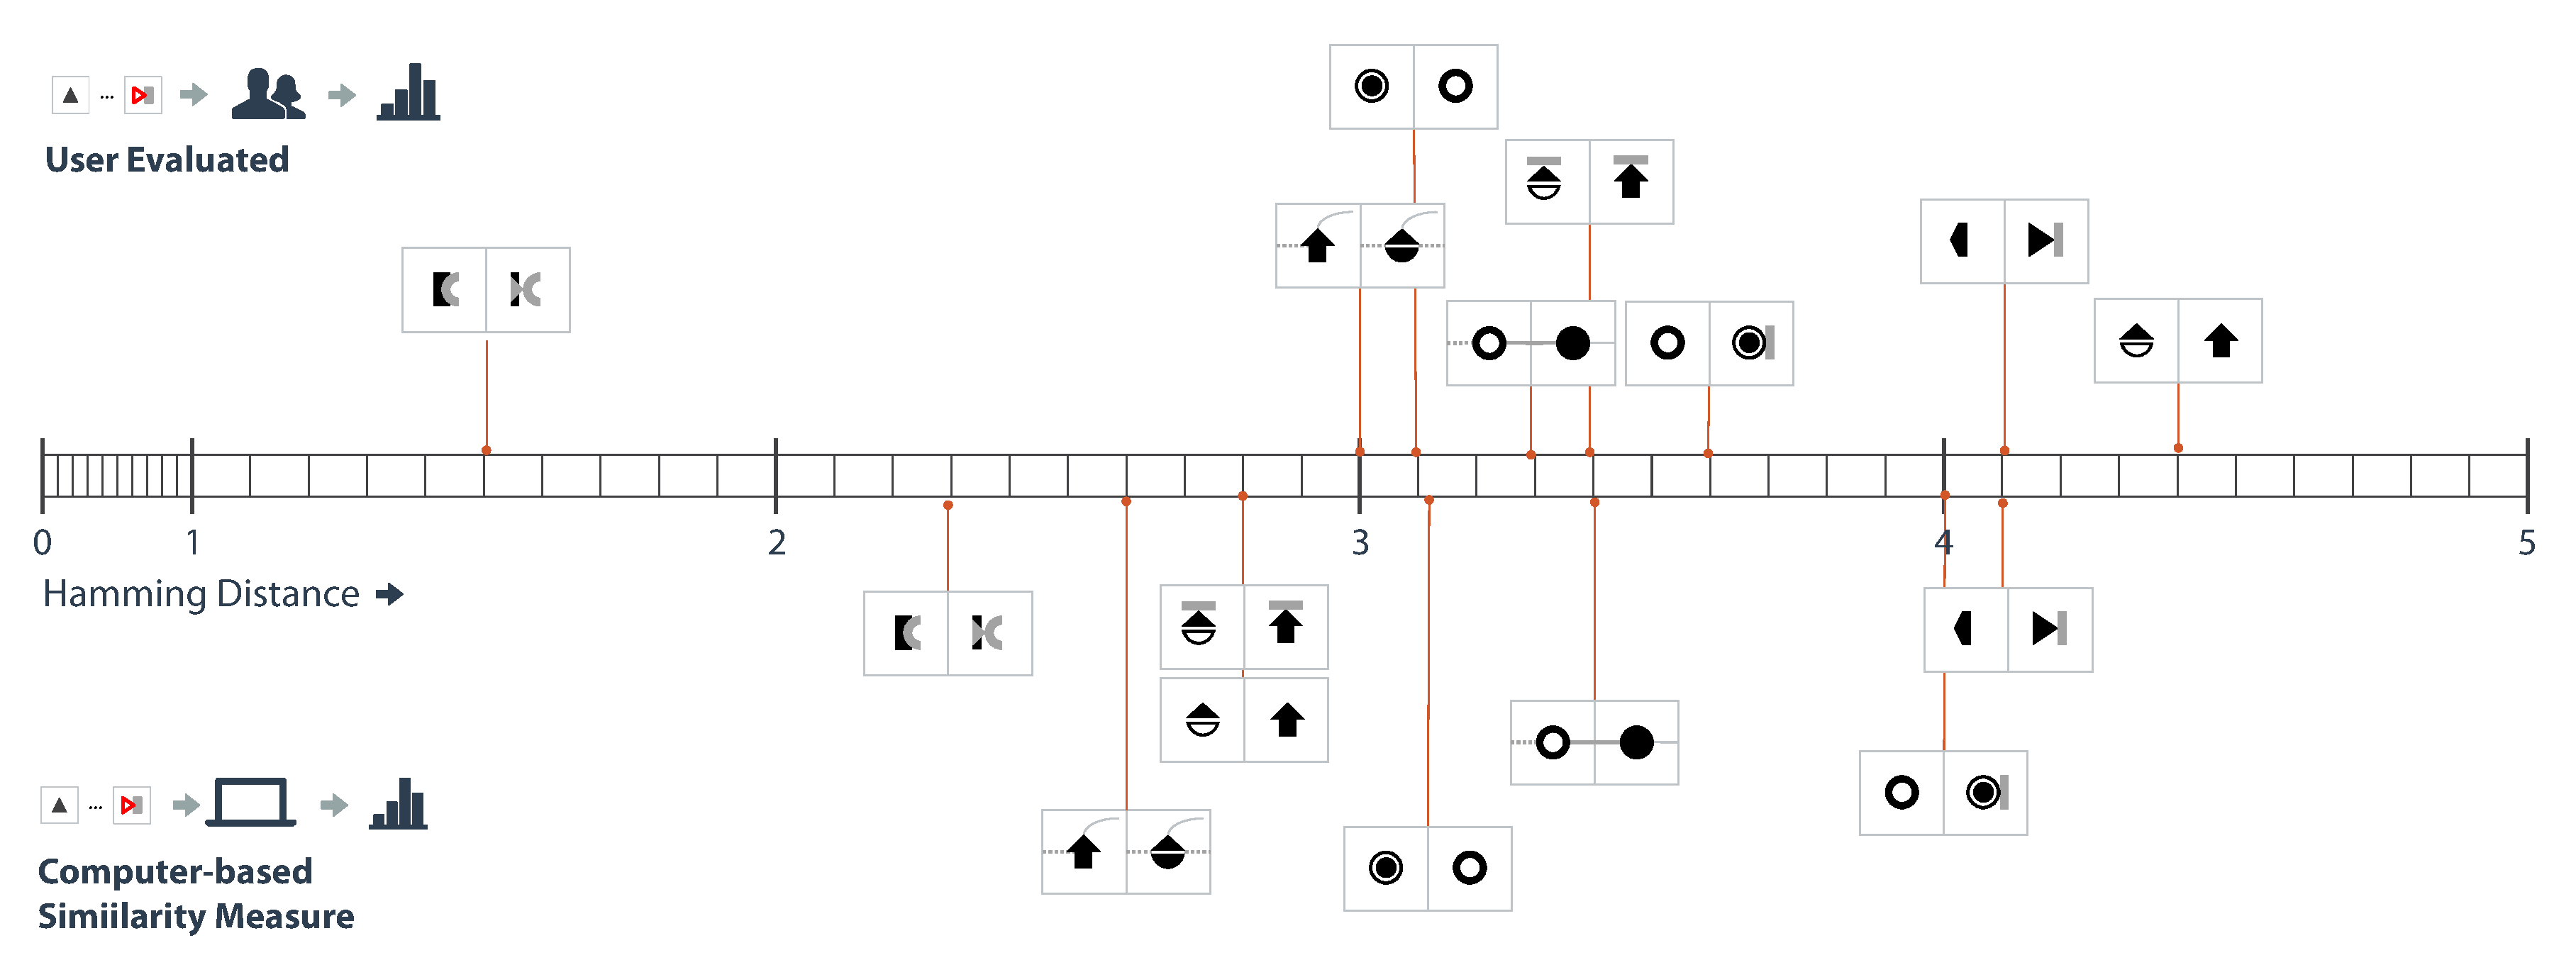
\includegraphics[width=\textwidth]{images/filesystem/Comparison_ourglyphs}
\end{center}
\caption{Sample of results for the file visualization glyph pairs used in both the user-centric estimation (top) and by computer-based similarity measure (bottom). Low values indicate difficult to differentiate and high values indicate easy to differentiate.}
\label{fig:our_glyph_scores}
\end{figure*}

The concept of the QHD has been considered throughout the design, development, evaluation, and application of the glyph-based file system visualization tool.
Our understanding and appreciation of this concept has improved along with this process.
Figure~\ref{table:fileoperations} shows eighteen glyphs for the most common events in file systems.
These events include creation, modification, deletion, copying, moving, and renaming.
These actions may be applied to a file, directory, device, shortcut (symbolic link), or meta-data.
The designs of these event glyphs evolved through several stages.

\textbf{Initial Design.} We first designed a set of glyphs in conjunction with the overall visual design of the visualization tool as shown in Figure~\ref{fig:system}.
This allowed us to appreciate how these glyphs may be used, and how glyph size for instance would affect the retinal variables that could be used.
Here we decided that the basic glyph design should not feature colour hue. 
This powerful retinal variable should be reserved show different users or to colour-code files or directories for example.

\textbf{Expert Estimation.} Four visualization researchers took part in this work, and all have publications in the area of glyph-based visualization.
Using knowledge from Chapter \ref{chap:glyph-tax} about different retinal variables and their properties, combined with our experience in glyph design, the original designs were improved.
This is similar to method 1 in Section~\ref{sec:qhd}.
We noticed that although we could reach agreement as to how easy or difficult it can be to differentiate pairs of glyphs, we could not easily agree on the reasons why.
When we explicitly tried to determine the QHD between a pair of glyphs, we were often influenced by many different features, component shapes, convexity, aspect ratio, curvature, and so on.
This experience led us to further appreciate the multi-faceted nature and the complexity in estimating the QHD.
For most of the glyphs in Figure~\ref{table:fileoperations}, their designs stabilized at this stage. 

\textbf{Crush Tests.} We applied crush tests to all glyphs designed during the case study.
In several cases, we carried out systematic testing by applying consistent zooming factors to all glyphs.
Moreover, when considering individual glyphs, we carried out \emph{ad hoc} crush tests by using facilities in our drawing software, such as zooming, and overlaying a translucent shape on top of glyphs.
At this stage, we realized that simulating different conditions that would cause glyph quality to degenerate was not a trivial undertaking.
In many ways, this also echoed the multi-faceted nature and the complexity in estimating QHD as mentioned above.

\textbf{Human-centric Estimation.} We conducted a survey, partly to: gain a better understanding about the QHD in the context of individual retinal variables (see Section~\ref{sec:qhd}); and evaluate our event glyphs in Figure~\ref{table:fileoperations}.
We considered 20 different glyph designs, for which there would be one hundred and ninety pairwise comparisons.
We selected forty-eight pairs that were considered potentially more risky than other pairs.
We found that only one pair scored below two bits in terms of QHD in the survey.
The final designs of the glyphs did not include this pair.
The details of this evaluation will be given in Section~\ref{sec:eval_glyphs}.

\textbf{Computer-based Similarity Measures.} We used the same metric as mentioned in Section~\ref{sec:qhd} to measure the QHD of the forty-eight pairs that might be a risk.
We found that they all passed this QHD test.
The details of this evaluation will be also given in Section~\ref{sec:eval_glyphs}.

\textbf{Deployment in Software.} In addition to the above design efforts based on the concept of a QHD, we incorporated the glyph set into the visualization tool and used the tool to visualize events in a Dropbox folder and a Git repository.
This allowed us to gain direct experience about how these glyphs might be viewed and interpreted in practical applications.
The details of this deployment will be discussed in Section~\ref{sec:application}.

Differentiability is only one aspect of glyph design.
We have to consider other aspects such as how easy it is to learn and to remember glyphs, how glyphs may be connected, and how they may be ordered if the corresponding events happened to the same file or directory.
As shown in Figure~\ref{table:fileoperations}, we utilized some similar designs for files and directories to assist in learning and memorization.
Meanwhile, we also considered how they may be connected.
The three types of connection lines as shown at the top of the Figure~\ref{table:fileoperations}, and the different orientations shown in the third column may add additional features to help in glyph differentiation.
For example, all lines connecting to a \emph{deletion} glyph will always come from the left, and all connecting to a \emph{creation} glyph will extend to the right.
All lines connecting a \emph{copy} or \emph{move} glyph will suggest a spatial shift vertically.
In addition, semantic ordering, such as \emph{open} before \emph{read}, may also add extra differences to increase the QHD of the glyph designs as illustrated on the right side of Figure~\ref{table:fileoperations}.

\subsubsection{Evaluating Event Glyphs}
\label{sec:eval_glyphs}

%todo: show groups...%

We evaluated those glyphs in Figure~\ref{table:fileoperations} based on the QHD obtained from a human-centric survey and by using computer-based similarity measures.
We utilized the same survey and metrics as described in Section~\ref{sec:qhd} because this allowed us to compare the QHD for our glyph set against that for the reference pairs and primitives discussed in Section~\ref{sec:qhd}.
Note that for our glyphs only the potentially risky pairs were evaluated.

The human-centric estimation provided us with most meaningful insight about the quality of the glyphs.
The 104 pairs of glyphs evaluated by participants have an average QHD of 2.9 bits.
Figure \ref{fig:evaluation_groups} shows the 22 comparison groups used in this evaluation. 
The average QHD for the reference pairs (Groups A and B) is 2.7 bits.
The average for the primitive pairs (Groups C, D, E, F, G, H, I, J) is 2.6 bits.
The average for the potentially risky pairs in our file system glyph set (Groups O, P, Q, R, S, T, U, V, W, X, Y, Z) is 3.2 bits.
Almost all of our glyph pairs have their QHD above 2 bits, except one pair (QHD = 1.5 bits) which was not used in the final design.
The upper part of Figure~\ref{fig:eval_glyph_scores} shows a selection of the survey results.

Meanwhile, the computer-based metric also measured our glyph pairs favourably.
As mentioned in Section~\ref{sec:qhd}, the average QHD estimated by the metric is normalized to have the same min, mean and max as the human-centric estimation.
The complete set of 104 glyph pairs have an average QHD of 2.9 bits
The average QHD for the reference pairs is 2.6 bits.
The average for the primitive pairs is 2.7 bits.
The average for the potentially risky pairs in our glyph set is 3.1 bits.
The lowest QHD for our potentially risks glyph pairs is 2.1 bits.

\begin{figure*}[t!]
\begin{center}
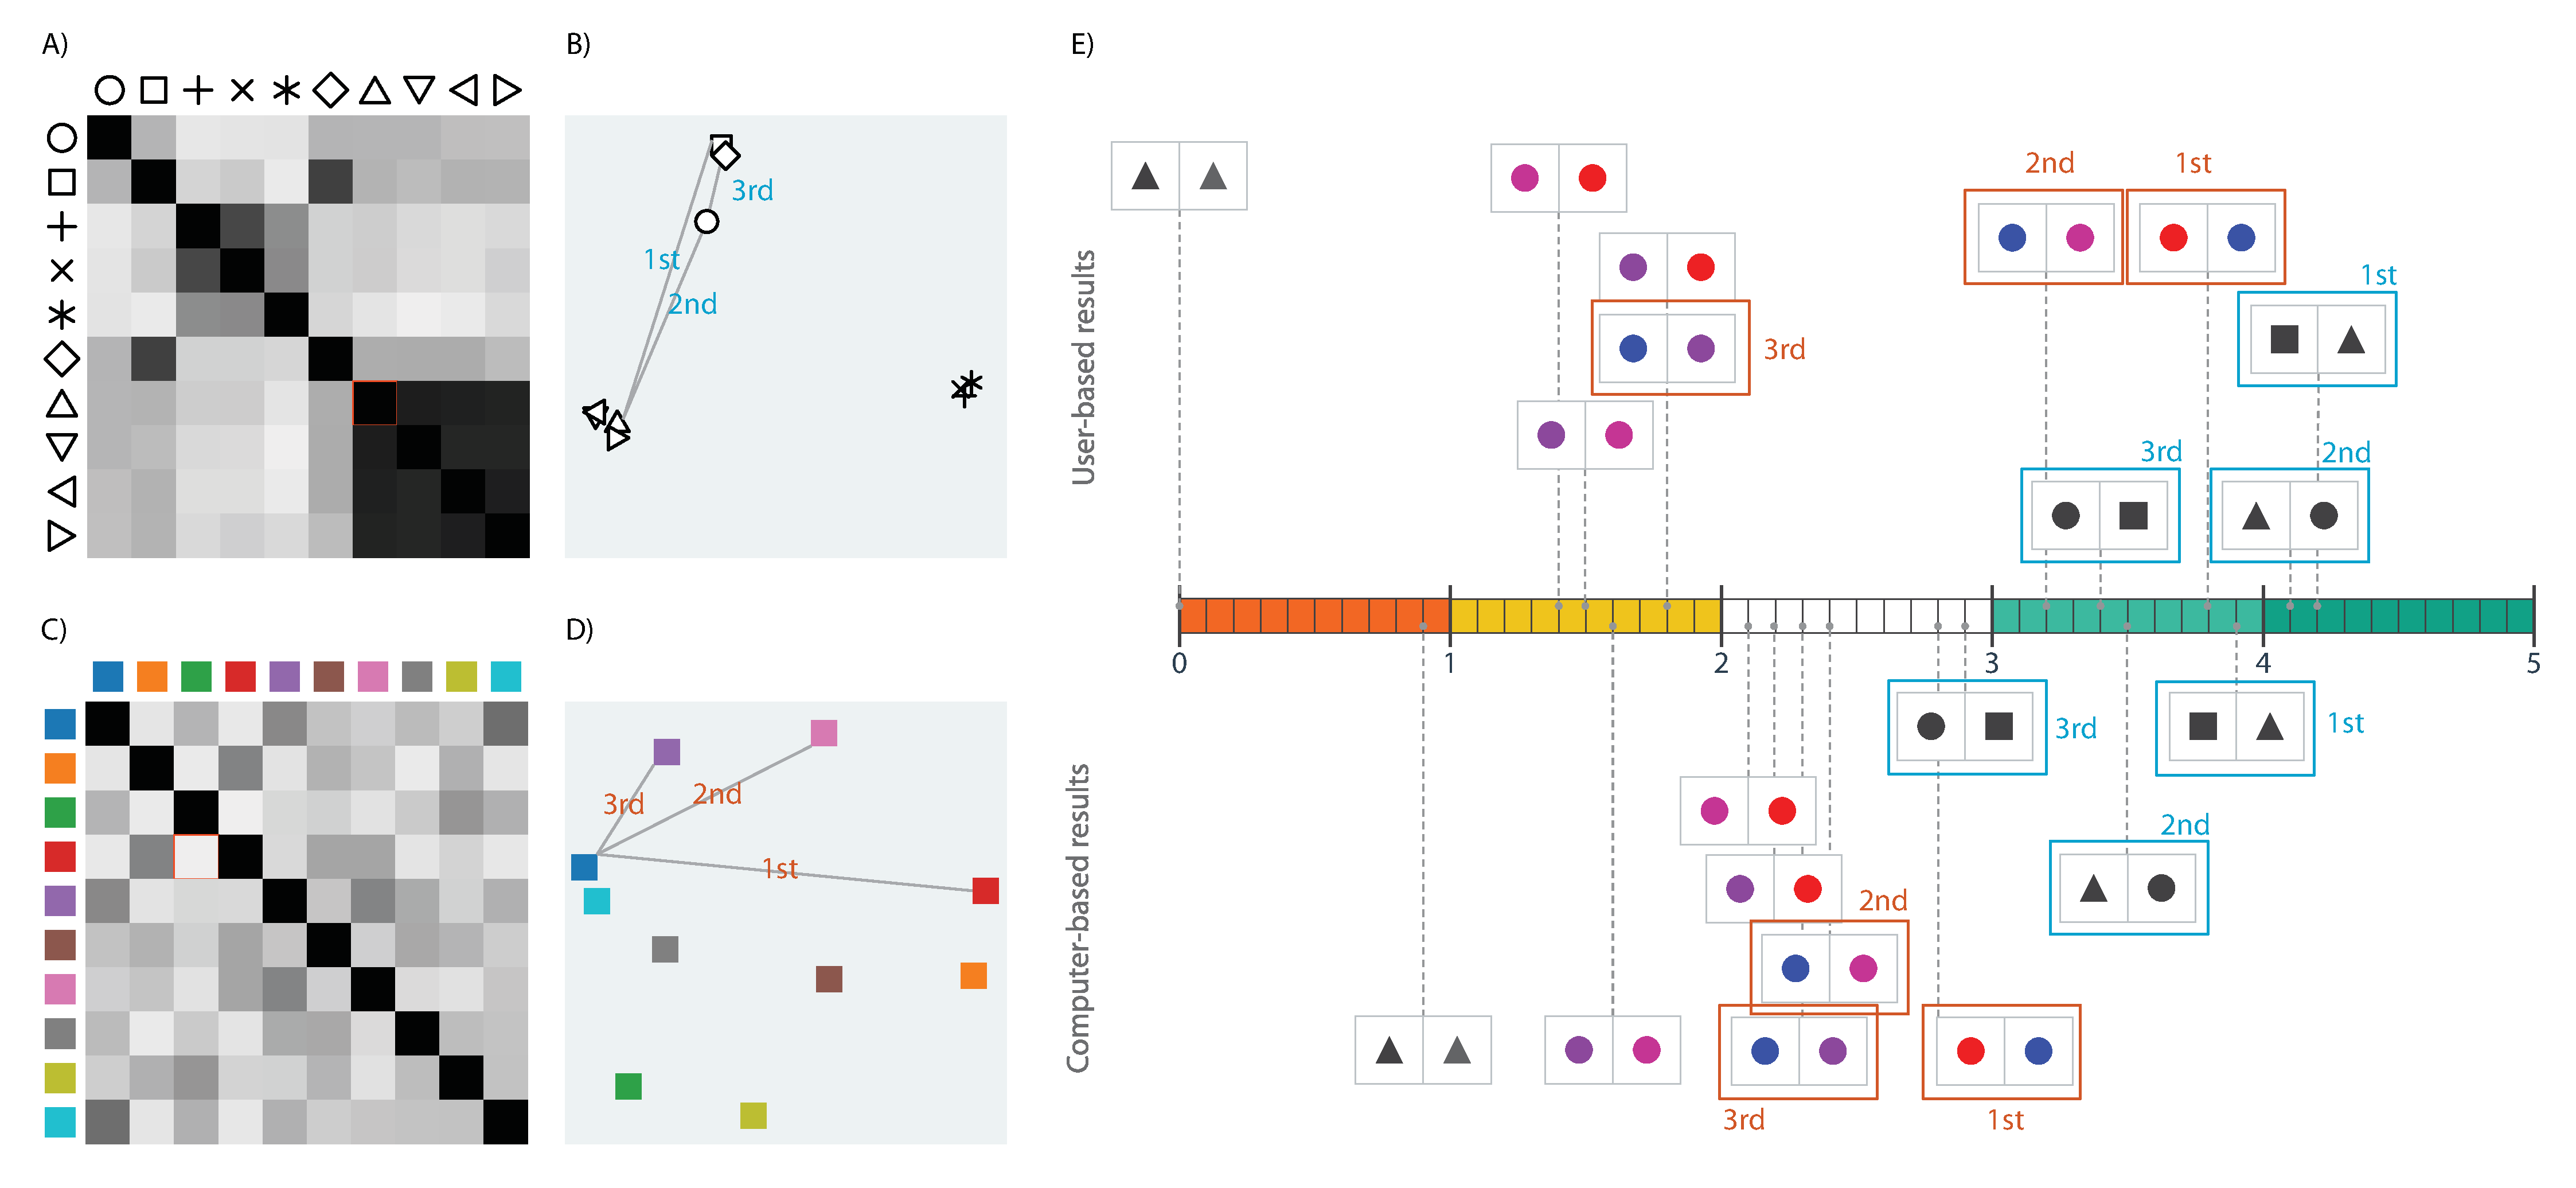
\includegraphics[width=\textwidth]{images/filesystem/perceptual_kernal_validation}
\end{center}
\caption{Results from crowd sourcing experiments by \cite{demiralplearning} (A-D) with respect to results from our analyses (E).
A) Distances between colours shown as a heat map.
The higher the similarity, the darker the square.
B) Shapes arranged by perceptual distance between them.
C) Distances between colours shown as a heat map.
D) Colours arranged by perceptual distance between them.
E) Results from our user-based and computation-based analyses.
The results are correlated with results from \cite{demiralplearning}.
The top three perceptually distant shapes and colours are marked across the results.}
\label{fig:perceptual_kernel}
\end{figure*}

Moreover, subsequent research presented by Demiralp \etal in their work on Perceptual Kernels\cite{demiralplearning} further validated our user-based and computer-based results.
Their findings for shape and colour distances are shown in Figure \ref{fig:perceptual_kernel} A - D.
These results are shown to be consistent with the overall results extrapolated from the user-based and computer-based metrics in Figure \ref{fig:perceptual_kernel} E. 

The evaluation also showed some interesting phenomena.
The additional features added to the directory glyphs have reduced QHD among directory glyphs.
For example, when comparing Group O and Group Q, where the glyphs for \emph{creation}, \emph{modify metadata}, and \emph{modify content} were compared within the context of files and directories respectively, human-centric estimation shows a noticeable difference.
The average QHD for Group O (files) is 3.4 bits and that for Group Q (directories) is 2.6 bits.
Similarly, for Group T and Group V where \emph{move}, \emph{copy}, and \emph{short cut} glyphs were compared, the average QHD for Group T (files) is 3.3 bits, and that for Group V (directories) is 2.8 bits.
Meanwhile, the computer-based similarity measures suggest little difference between O and Q and between T and V.
This suggests that further research is necessary to enrich the existing findings in perception about the distance functions for integrated and separable retinal variables~\cite{Maguire:2012:TVCG}.

\section{Examples: Dropbox and Git}
\label{sec:application}

To demonstrate the applicability of the above glyph encoding scheme, we developed an interactive visualization tool for visualizing event log data captured from two real world systems, Dropbox and Git.

Our glyph-based visualization software is comprised of two parts:
a) a back-end for processing commit logs of Dropbox and Git; and
b) a front-end serving as a web-based user interface as well as a software library;
The back end was written in Python.
It generates two types of JSON (JavaScript Object Notation) files for the front-end, one describing the directory structure and the other describing the events that occurred.
The front-end was created with a combination of HTML5, CSS and JavaScript (utilising Rapha\"{e}l.js\footnote{http://raphaeljs.com} for the visualization element and jQuery).
The glyphs are stored as a font created using IcoMoon\footnote{http://icomoon.io}.

In addition to glyph-based visualization, the system supports a variety of interactions including:
%
\begin{itemize}
\item Filtering different types of file system events;
\vspace{-3mm}
\item Filtering different users;
\vspace{-3mm}
\item Selecting a specific directory as a subtree;
\vspace{-3mm}
\item Selecting different time period;
\vspace{-3mm}
\item Zooming, and scrolling along both the directory axis and the time line; and
\vspace{-3mm}
\item Showing a detailed pop up window when the mouse hovers over an event glyph.
\end{itemize}

\subsection{Visualizing Dropbox Activity Logs}

\begin{figure*}[ht!]
\begin{center}
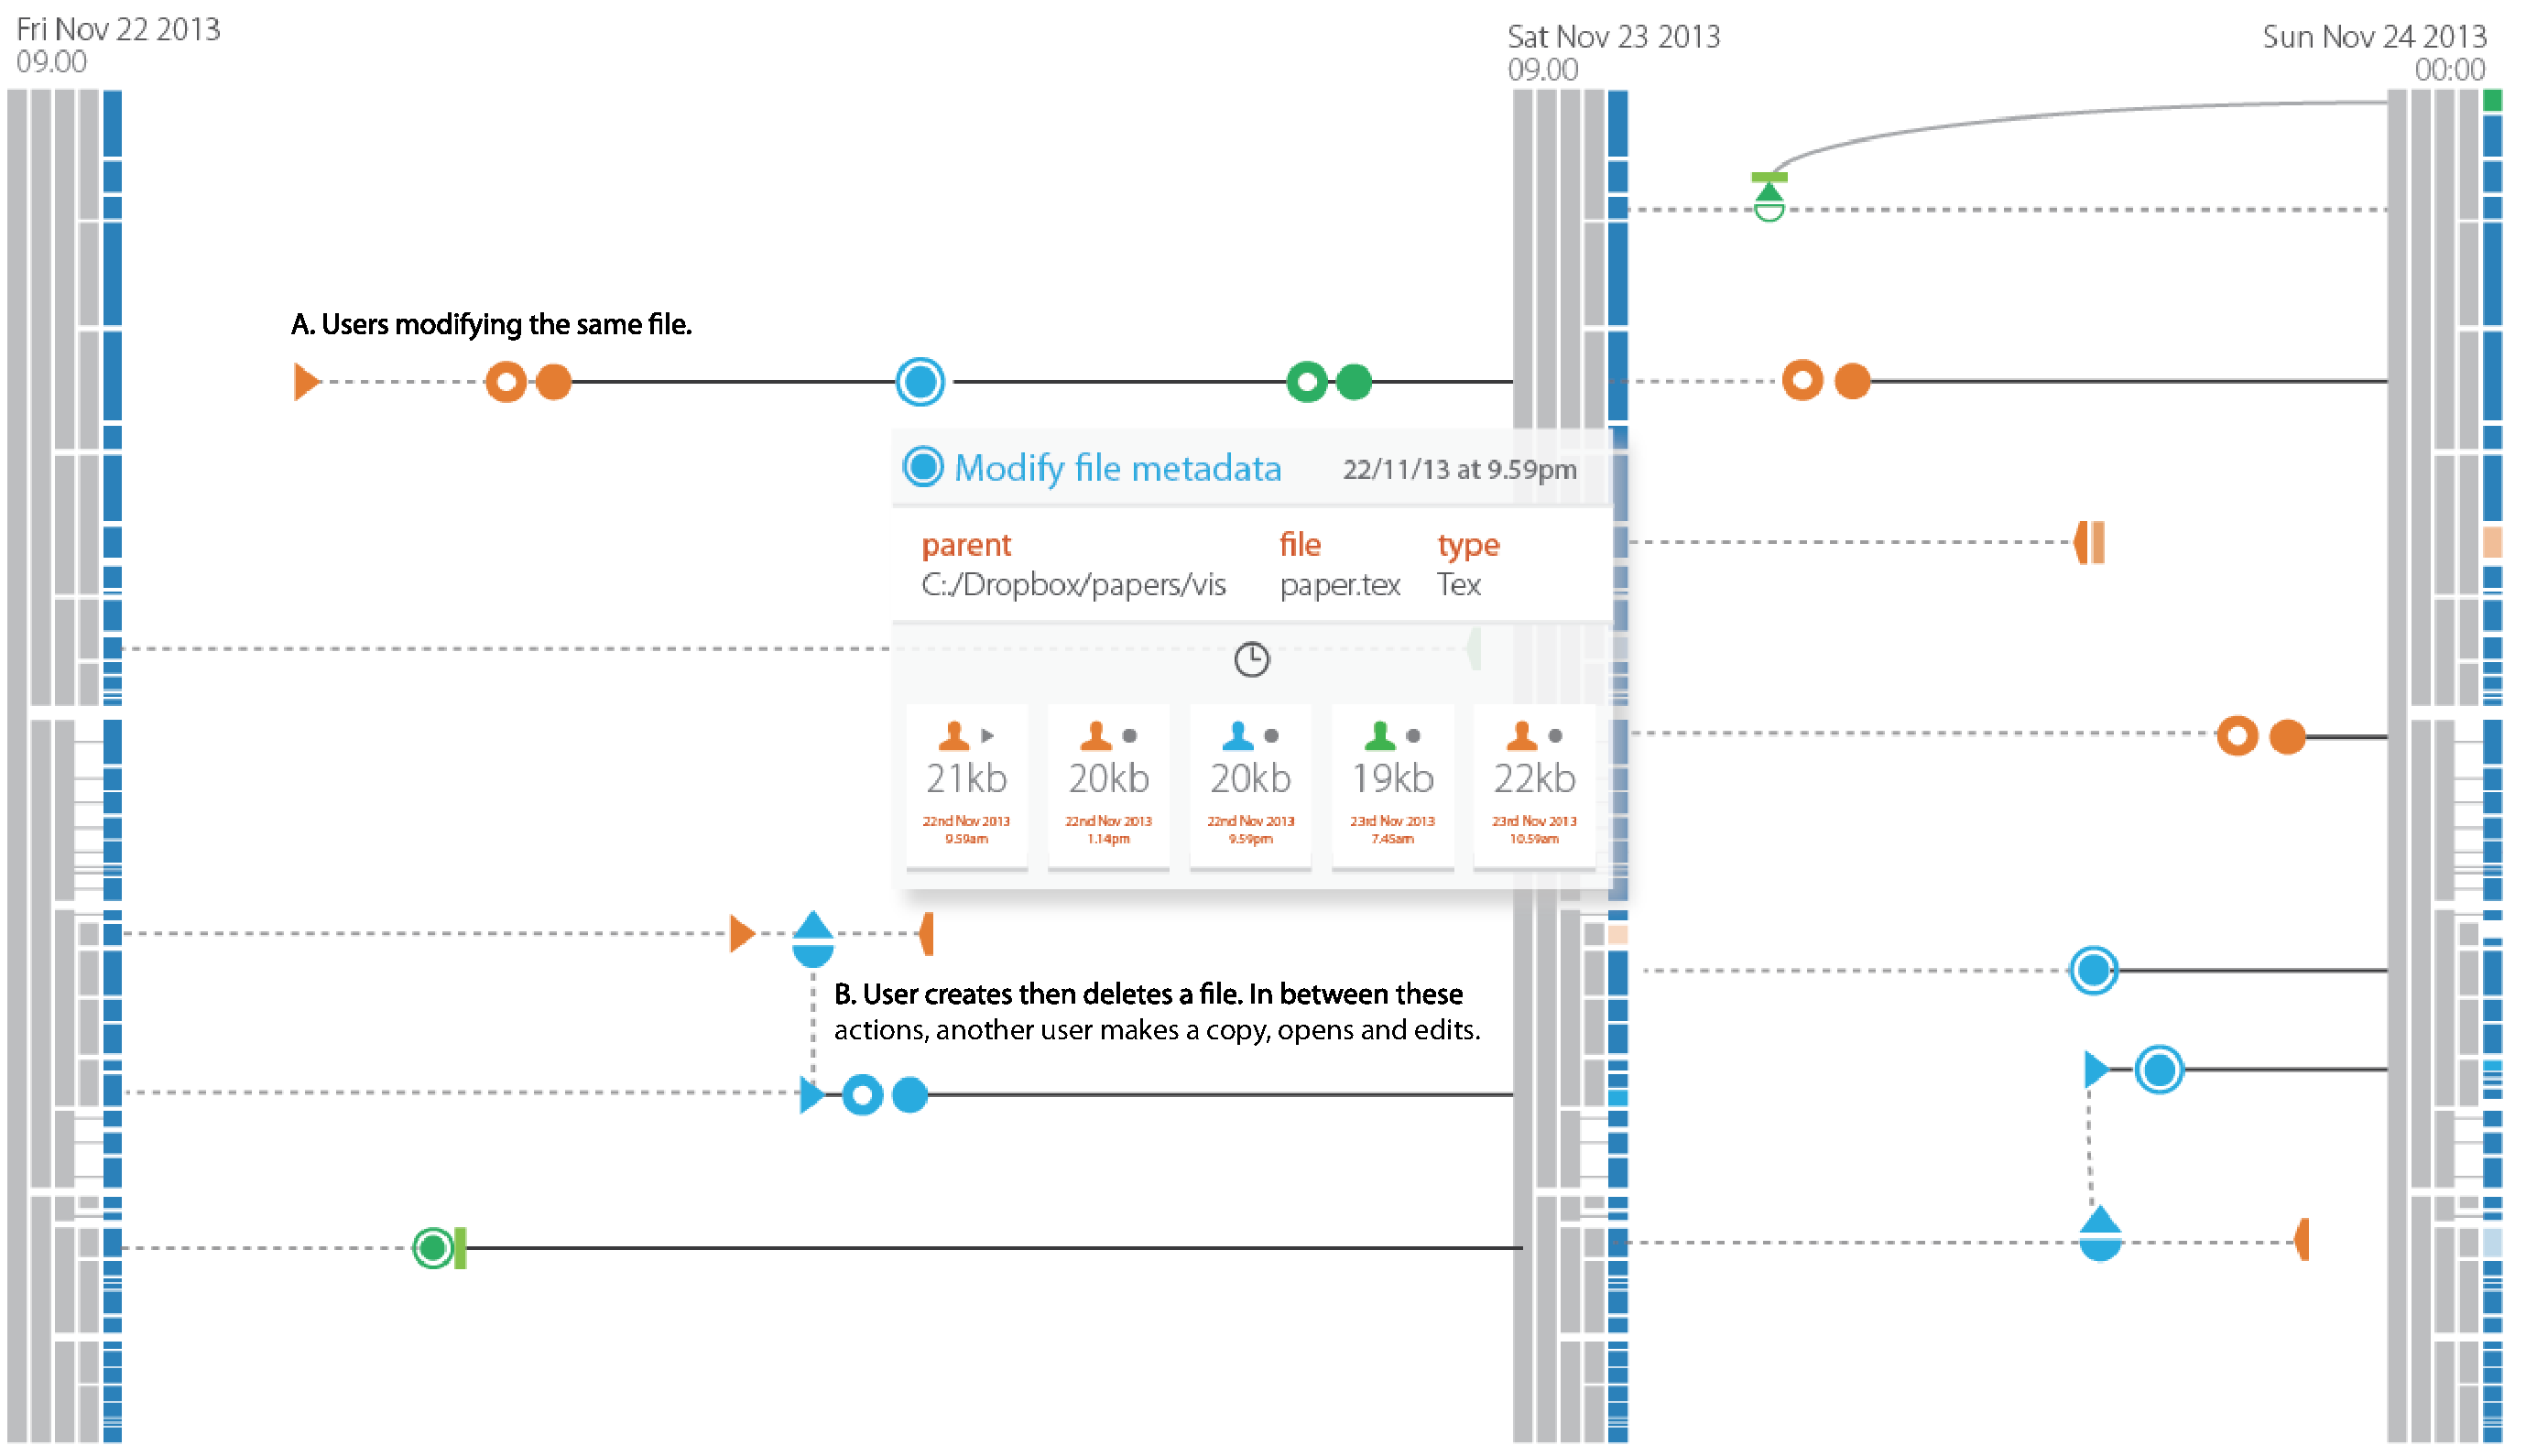
\includegraphics[width=\textwidth]{images/filesystem/dropbox-casestudy-2}
\end{center}
\caption{Glyph-based visualization is used to display events from a Dropbox activity log. The vertical bars are an abstract representation a directory tree and the timeline flows from left to right.
In event A) we can see the case where a number of users have been modifying the same file. The popup gives more details about the modifications, who did them and when. This allows for provenance tracking where such information is available.
In event B) we have another case where \emph{user X} (orange) creates a file, then \emph{user Y} creates a copy of this file, opens it and modifies its contents. \emph{User X} then deletes the original file, however a modified copy exists elsewhere.}
\label{fig:dropbox}
\end{figure*}

%
Dropbox is a popular cloud service that allows users to synchronize their files across multiple devices.
It allows users to create shared directories that other users can be invited to access.
This makes it especially useful for collaborative activities between institutions and colleagues, and for sharing personal media with family and friends.
Because of its file sharing capability, it is desirable for users to visualize events in a shared folder, for instance, to see which file has been created or modified recently and by whom.
Although the service does provide a text-based activity log that users can access, it is time-consuming and tedious to read a long list of events.


As shown in Figure~\ref{fig:dropbox}, a glyph-based visualization allows users to gain an overview of the events in a shared folder with ease.
As discussed previously, we colour was avoided in the initial glyph design.
This means that the visualization system can encode information, such as different users, or different types of files with colour.
In Figure~\ref{fig:dropbox}, colours are used to depict different users.
We can observe that three different users have accessed the system during this displayed period (shown by the blue, orange, and green glyphs).
Going back to what was presented in Chapter \ref{chap:related_work}, the number of colours that can be used in a visualization is limited (8-12).
When the number of colours increases, the number of errors will increase.
At this point, a smaller number of categories would be created for users to reduce the number of colours required, \eg, user groups, location, and so on.

The three vertical bars are simplified views of the directory tree concerned.
It is a fairly large directory with three further levels of sub-directories.
The period displayed spans over 39 hours, and a variety of events took place.
Some indicate close collaboration, when a line of activities linked different users to a single file.
For example, the top line in the left half section shows that the orange user created a file, and then opened and modified it.
After several hours, the blue user modified the metadata of the file (possibly renaming it or changing its access date).
Several hours later, the green user opened and modified it.
If a viewer wishes inspect an event in detail, or simply forget the meaning of a glyph, he/she can simply hovers the mouse over the glyph and a pop-up window will display details about the event and the file or directory concerned.
The detailed information includes the filename, the parent directory, and the file type.
It also shows file-specific history, such as the operations that each user performed and the file size after each operation.
Collaborative colleagues can become aware of ongoing actions, reducing the need to inform each other of every file access action via email.

\subsection{Visualizing Git Repository History}
%

\begin{figure*}[ht!]
\begin{center}
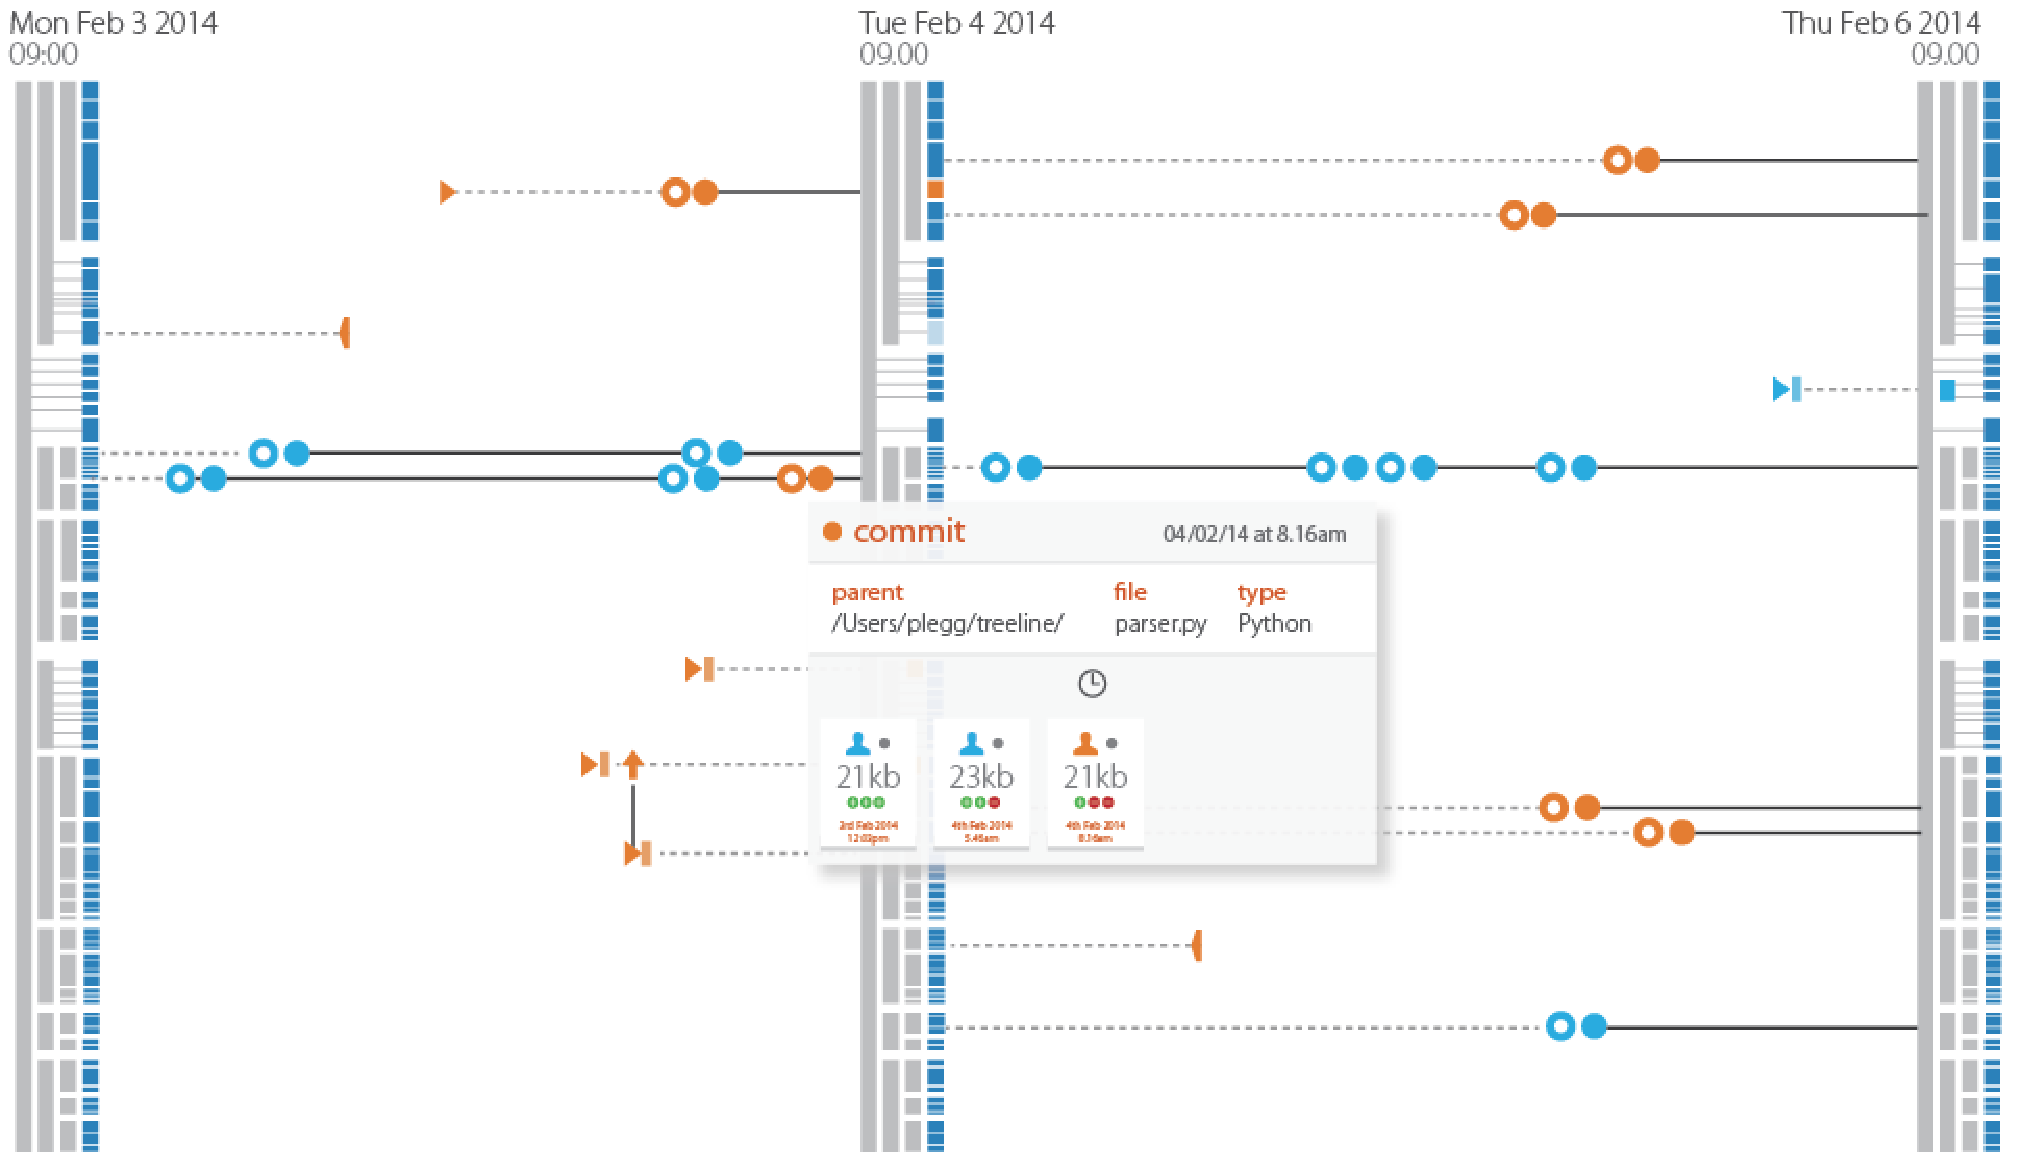
\includegraphics[width=\textwidth]{images/filesystem/git-casestudy-2}
\end{center}
\caption{Glyph-based visualization is used to display events in the history data of a Git repository, where two co-developers were actively working on different parts of the software. They distributed their effort in a coordinated manner, so as to avoid conflicts and problems when merging code. Only on one occasion, \emph{user X} (orange) has modified a file in an area of the repository normally occupied by \emph{user Y} (blue). We can also see that \emph{user X} has been most active when it comes to creating and deleting directories/files compared to \emph{user Y} who has been more active in terms of editing and committing files.}
\label{fig:git}
\end{figure*}

Git is a distributed version control system, allowing programmers to develop software in a collaborative manner.
It was first released in 2005, and became popular among programmers after the launch of web-based hosting services such as GitHub \footnote{\url{www.github.com}}.
The main file storage is known as the repository, and users can pull from, or push to, the repository from their local version of the Git file storage.
Although Git maintains a comprehensive history of file access and revision for a repository, it is time-consuming for Git users to read the history data of a Git repository.
Glyph-based visualization can offer an efficient means to gain a quick overview of such history data.

Figure~\ref{fig:git} shows an example visualization of a shared repository between two of the co-authors of this work.
As both users in this collaboration had a good understanding of the joint software development project, they only need a quick glance at the visualization to get a sense of the ongoing programming effort by each member of the team.
In comparison to reading the repository history, the visualization provides a much more efficient and effective means for their ``silent communication'' and ``autonomous coordination''.
It is also easy for any one of the co-developers to see major actions, such as deleting a file.
From Figure~\ref{fig:git}, one can quickly identify two file deletion actions, one around 17:00 on Monday and one around 17:00 on Tuesday.
Additionally, such a visualization can show where effort is being placed on different modules of the software.
This is not easily achieved through current tools. 
For example, for a new ``feature'' in development, one may expect users to only work within a particular area of the code base. 
Working outside those areas may point to some unnecessarily ``tight coupling'' (close dependency between modules) that could be removed to make the software better designed.


\section{Contributions}
\label{sec:conclusion}
%
In this chapter, we have presented a novel conceptual framework, based around the \emph{quasi-Hamming distance} (QHD), which facilitates a systematic approach to the design of fail-safe glyph encoding schemes.
As the conceptual framework is built on well-proven theories and practice in communication, it offers the potential to stimulate further research on this topic with a depth and breadth comparable to the topic of error detection and error correction in communication.
To demonstrate the feasibility of this conceptual framework, we presented two proof-of-concept experiments, where we obtained QHD measures from a human-centric survey and from computer-based similarity measures.
To demonstrate its practical applicability, we conducted a case study where event logs from Dropbox and Git were visualized using a set of fail-safe glyphs.
From the very beginning, the glyph set was designed to ensure a high-level of differentiability, while accommodating requirements such as minimal colour use and metaphoric consistency.
The glyphs were evaluated using QHD measures obtained from a human-centric survey and computer-based similarity measures.
These results were validated using research.

This work is very much a first step towards the establishment of a collection of mathematical and cognitive theories, experimental findings and statistics, design techniques and computational metrics for guiding, and aiding glyph designs.
This work highlights a number of gaps, where further research is needed.
For example, it is highly desirable for us to understand the relationship between the JND measures of various retinal variables and differentiability of glyphs encoded using such retinal variables.
It is also highly desirable to research into computer-based similarity measures that are statistically closer to human-centric estimation.